\documentclass{report}
\usepackage{graphicx}
\graphicspath{{./images/}}
\begin{document}
\subsection{Description de l'extension}

Cette extension a pour but de permettre aux clients de passer à une version premium de l'application désignée pour les entreprises ou les organisations afin de gérer leurs divisions et bâtiments sous une forme hiérarchique.

\\\\\\
\subsection{Use Case Diagram}
\subsubsection{Description des use cases}
\noindent \\
\begin{tabular}{|r|p{9cm}|}
    \hline
    Titre: & Buy subscription \\
    \hline
    Description : & L'utilisateur veut acheter un abonnement. \\
    \hline
    Acteur(s) principal(aux) : & Client. \\
    \hline
    Précondition : & Le client est sur la page principale de l'application. \\
    \hline
    Post condition : & Le client est sur la page de confirmation d'achat. \\
    \hline
    Scénario principal : & \begin{enumerate}[left=0pt, topsep=0pt]
        \item le client clique sur le bouton d'achat d'abonnement
        \item le client introduit ses informations bancaires pour le payement
        \item l'application vérifie que les informations entrées sont correctes 
        \item le payement est procédé
        \item le compte du client passe en version premium et le client est notifié 
    \end{enumerate} \nointerlineskip \\
    \hline
    Scénario alternatif : & lors du payement, les informations bancaires sont incorrectes 
    \begin{enumerate}[left=0pt, topsep=0pt]
    		\item l'application prévient le client que ses informations sont incorrectes
    \end{enumerate} \nointerlineskip \\
    \hline
    Trigger : & Lorsque l'utilisateur clique sur le bouton \textbf{upgrade to pro version}. \\
    \hline
    Fréquence d'utilisation : & Peu fréquent. \\
    \hline
\end{tabular}
\\\\\\
\begin{tabular}{|r|p{9cm}|}
    \hline
    Titre: & Renew subscription \\
    \hline
    Description : & Le client souhaite rallonger son abonnement. \\
    \hline
    Acteur(s) principal(aux) : & Client premium. \\
    \hline
    Précondition : & Le client est sur la page principale de l'application et il est déjà premium. \\
    \hline
    Post condition : & Le client est sur la page de confirmation du renouvellement de l'abonnement. \\
    \hline
    Scénario principal : & \begin{enumerate}[left=0pt, topsep=0pt]
        \item le client clique sur le bouton d'achat d'abonnement
        \item le client introduit ses informations bancaires
        \item l'application vérifie que les informations entrées sont correctes 
        \item le payement est procédé
        \item l'abonnement du client est rallongé et il est notifié
    \end{enumerate} \nointerlineskip\\
    \hline
    Scénario alternatif : & lors du payement, les informations bancaires sont incorrectes 
    \begin{enumerate}[left=0pt, topsep=0pt]
    		\item l'application prévient le client que ses informations sont incorrectes
    \end{enumerate} \nointerlineskip \\
    \hline
    Trigger : & Lorsque l'utilisateur clique sur le bouton \textbf{renew subscription} \\ 
    \hline
    Fréquence d'utilisation : & Peu fréquent. \\
    \hline
\end{tabular}
\\\\\\
\begin{tabular}{|r|p{9cm}|}
    \hline
    Titre: & Create division \\
    \hline
    Description : & Le client souhaite créer une division. \\
    \hline
    Acteur(s) principal(aux) : & Client premium ou division d'entreprise. \\
    \hline
    Précondition : & Le client est sur la page listant ses divisions. \\
    \hline
    Post condition : & Le client est sur la page listant ses divisions. \\
    \hline
    Scénario principal : & \begin{enumerate}[left=0pt, topsep=0pt]
        \item Le client clique sur le bouton pour ajouter une division
        \item Le client introduit les informations de la division
        \item La division est rajouté au  compte 
    \end{enumerate} \nointerlineskip\\
    \hline
    Trigger : & Lorsque l'utilisateur clique sur le bouton \textbf{Add division} \\ 
    \hline
    Fréquence d'utilisation : & Peu fréquent. \\
    \hline
\end{tabular}
\\\\\\
\begin{tabular}{|r|p{9cm}|}
    \hline
    Titre: & Delete division \\
    \hline
    Description : & Le client souhaite supprimer une division. \\
    \hline
    Acteur(s) principal(aux) : & Client premium ou division d'entreprise. \\
    \hline
    Précondition : & Le client est sur la page des divisions. \\
    \hline
    Post condition : & Le client est sur la page des divisions. \\
    \hline
    Scénario principal : & \begin{enumerate}[left=0pt, topsep=0pt]
        \item le client clique sur la division
        \item le client clique sur le bouton supprimer
        \item le client confirme son choix
        \item la division choisie est supprimée et le client est notifié 
    \end{enumerate} \nointerlineskip\\
    \hline
    Trigger : & Lorsque l'utilisateur clique sur le bouton \textbf{Delete division} \\ 
    \hline
    Fréquence d'utilisation : & Peu fréquent. \\
    \hline
\end{tabular}
\\\\\\
\begin{tabular}{|r|p{9cm}|}
    \hline
    Titre: & Modify division \\
    \hline
    Description : & Le client souhaite modifier une division. \\
    \hline
    Acteur(s) principal(aux) : & Client premium ou division d'entreprise. \\
    \hline
    Précondition : & Le client est sur la page des divisions. \\
    \hline
    Post condition : & Le client est sur la page des divisions. \\
    \hline
    Scénario principal : & \begin{enumerate}[left=0pt, topsep=0pt]
        \item le client clique sur la division
        \item le client clique sur le bouton modifier
        \item le client modifie les informations de la division
        \item le client confirme son choix
        \item la division choisie est modifiée et le client est notifié 
    \end{enumerate} \nointerlineskip\\
    \hline
    Trigger : & Lorsque l'utilisateur clique sur le bouton \textbf{edit division} \\ 
    \hline
    Fréquence d'utilisation : & Peu fréquent. \\
    \hline
\end{tabular}
\\\\\\
\begin{tabular}{|r|p{9cm}|}
    \hline
    Titre: & View division consumption \\
    \hline
    Description : & Le client souhaite voir la consommation une division. \\
    \hline
    Acteur(s) principal(aux) : & Client premium ou division d'entreprise. \\
    \hline
    Précondition : & Le client est sur la page des divisions. \\
    \hline
    Post condition : & Le client est sur la page des informations de consommation de la division. \\
    \hline
    Scénario principal : & \begin{enumerate}[left=0pt, topsep=0pt]
        \item le client clique sur la division
        \item le client est sur la page de la consommation de la division 
    \end{enumerate} \nointerlineskip\\
    \hline
    Trigger : & Lorsque l'utilisateur clique sur le bouton de la division \\ 
    \hline
    Fréquence d'utilisation : & Fréquent. \\
    \hline
\end{tabular}
\\\\\\
\begin{tabular}{|r|p{9cm}|}
    \hline
    Titre: & Add building \\
    \hline
    Description : & Le client souhaite ajouter un bâtiment à une division. \\
    \hline
    Acteur(s) principal(aux) : & Client premium ou division d'entreprise. \\
    \hline
    Précondition : & Le client est sur la page de la division. \\
    \hline
    Post condition : & Le client est sur la page de la division. \\
    \hline
    Scénario principal : & \begin{enumerate}[left=0pt, topsep=0pt]
        \item le client clique sur le bouton d'ajout de batiment
        \item le client introduit les informations du batiment
        \item le batiment est rajouté à la division et le client est notifié 
    \end{enumerate} \nointerlineskip\\
    \hline
    Trigger : & Lorsque l'utilisateur clique sur le bouton \textbf{add building} \\ 
    \hline
    Fréquence d'utilisation : & Peu fréquent. \\
    \hline
\end{tabular}
\\\\\\
\begin{tabular}{|r|p{9cm}|}
    \hline
    Titre: & Remove building \\
    \hline
    Description : & Le client souhaite supprimer le bâtiment de la division. \\
    \hline
    Acteur(s) principal(aux) : & Client premium ou division d'entreprise. \\
    \hline
    Précondition : & Le client est sur la page des bâtiments de la division. \\
    \hline
    Post condition : & Le client est sur la page des bâtiments de la division. \\
    \hline
    Scénario principal : & \begin{enumerate}[left=0pt, topsep=0pt]
        \item le client clique sur le bouton du bâtiment
        \item le client clique sur le bouton pour supprimer le batiment
        \item le client confirme son choix
        \item le bâtiment est supprimé et le client est notifié 
    \end{enumerate} \nointerlineskip\\
    \hline
    Trigger : & Lorsque l'utilisateur clique sur le bouton \textbf{remove building} \\ 
    \hline
    Fréquence d'utilisation : & Peu fréquent. \\
    \hline
\end{tabular}
\\\\\\
\begin{tabular}{|r|p{9cm}|}
    \hline
    Titre: & Modify building \\
    \hline
    Description : & Le client souhaite modifier les informations du bâtiment de la division. \\
    \hline
    Acteur(s) principal(aux) : & Client premium ou division d'entreprise. \\
    \hline
    Précondition : & Le client est sur la page des bâtiments de la division. \\
    \hline
    Post condition : & Le client est sur la page des bâtiments de la division. \\
    \hline
    Scénario principal : & \begin{enumerate}[left=0pt, topsep=0pt]
        \item le client clique sur le bouton du bâtiment
        \item le client clique sur le bouton pour modifier le bâtiment
        \item le client change les informations du bâtiment
        \item le bâtiment est modifié et le client est notifié 
    \end{enumerate} \nointerlineskip\\
    \hline
    Trigger : & Lorsque l'utilisateur clique sur le bouton \textbf{modify building} \\ 
    \hline
    Fréquence d'utilisation : & Peu fréquent. \\
    \hline
\end{tabular}
\\\\\\
\begin{tabular}{|r|p{9cm}|}
    \hline
    Titre: & View building consumption \\
    \hline
    Description : & Le client souhaite voir la consommation du bâtiment de la division. \\
    \hline
    Acteur(s) principal(aux) : & Client premium ou division d'entreprise. \\
    \hline
    Précondition : & Le client est sur la page des bâtiments de la division. \\
    \hline
    Post condition : & Le client est sur la page de la consommation de la division. \\
    \hline
    Scénario principal : & \begin{enumerate}[left=0pt, topsep=0pt]
        \item le client clique sur le bouton du bâtiment
        \item le client est sur la page avec la consommation du bâtiment
    \end{enumerate} \nointerlineskip\\
    \hline
    Trigger : & Lorsque l'utilisateur clique sur le bouton du bâtiment \\ 
    \hline
    Fréquence d'utilisation : & Fréquent. \\
    \hline
\end{tabular}
\\\\\\
\newpage
\subsubsection{Image de l'Use Case Diagram}
Voici le Use Case Diagram avec les différents Use Cases rajoutés pour l'extension.
\begin{figure}[h]
	\centering
	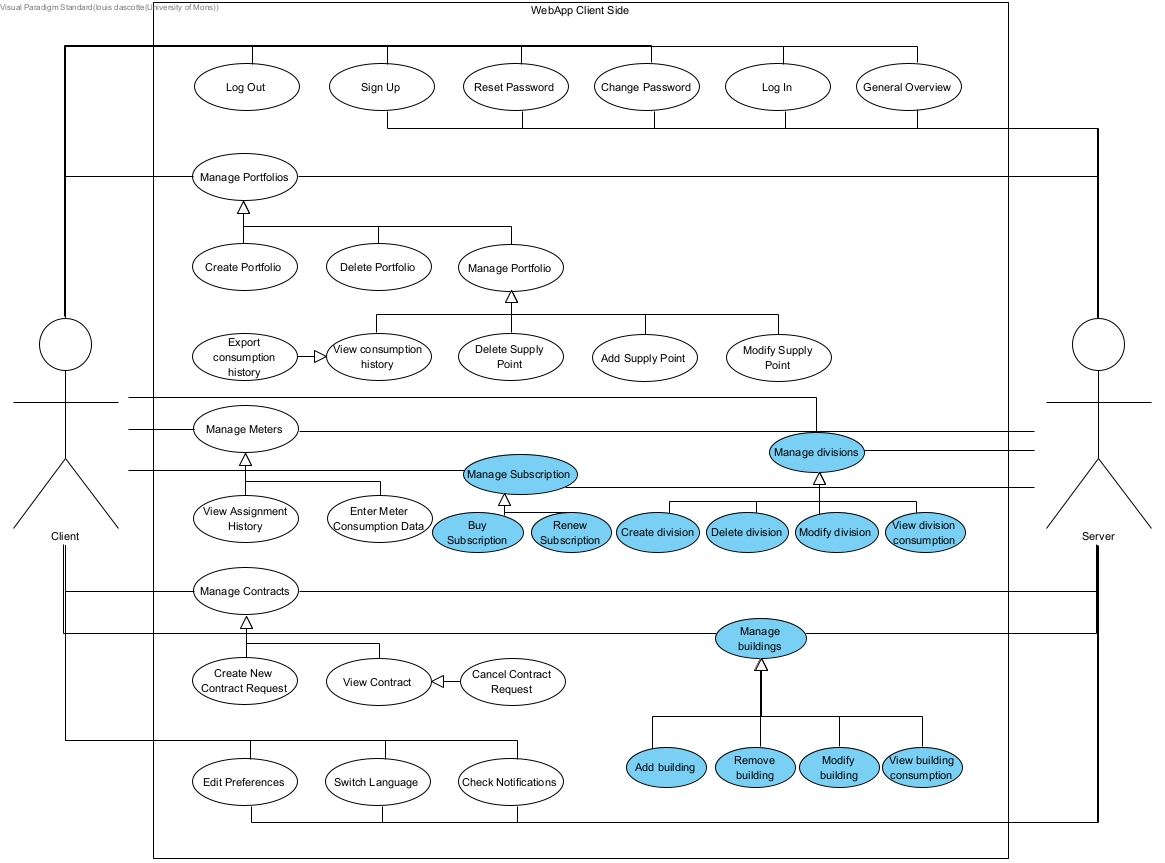
\includegraphics[width=1.3\textwidth]{UCD Client}
	\caption{Use Case Diagram}
	\label{fig:usdClient}
\end{figure}

\subsection{Sequence Diagram}
\subsubsection{Upgrade account}
Le diagramme de séquence ci-dessous représente comment un compte passe en version premium ou une extension de l'abonnement. \\
Si les informations bancaires sont correctes, on a deux options. Soit on a un compte pas encore premium, et donc il va passer en version pro. Sinon on a un compte déjà pro qui va étendre la durée de son abonnement.\\
\begin{figure}[h]
	\centering
	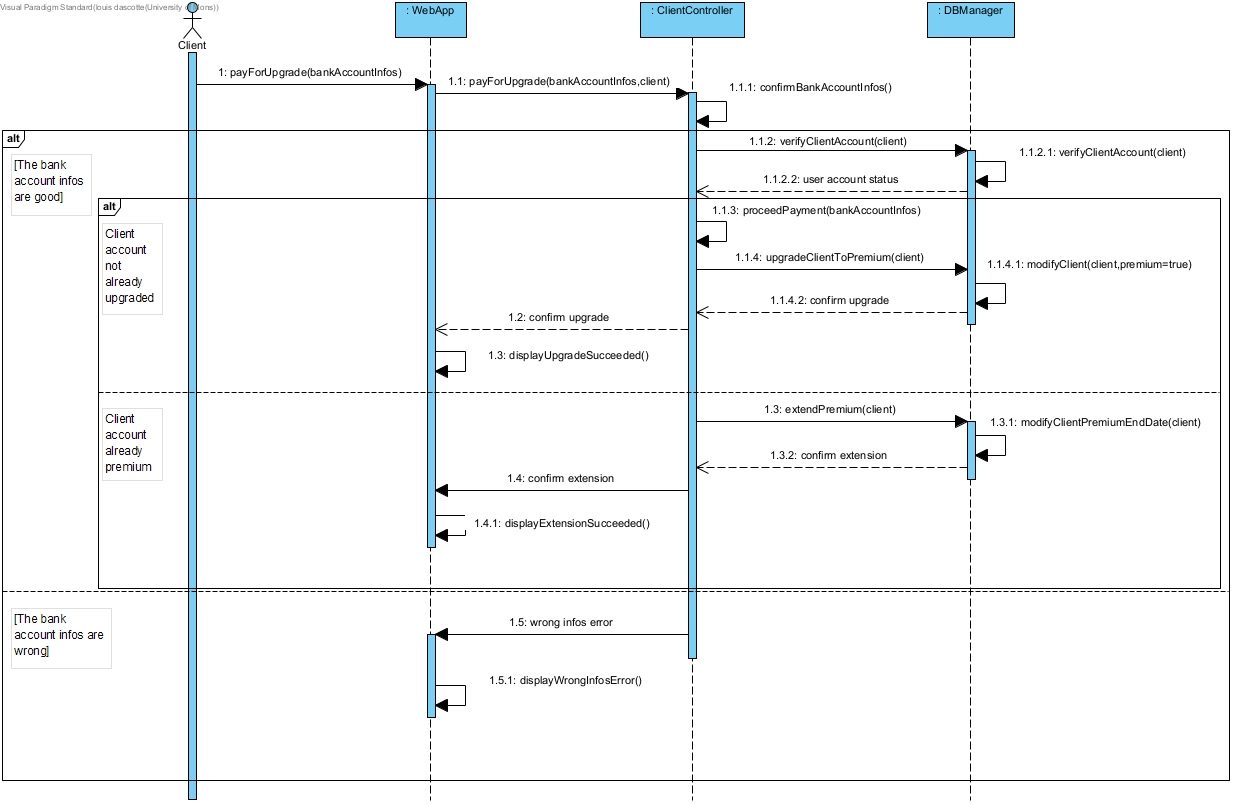
\includegraphics[width=1.3\textwidth]{upgrade account}
	\caption{Sequence Diagram}
	\label{fig:upgrade}
\end{figure}

\newpage
\subsection{Interaction Overview Diagram}
\begin{figure}[h]
	\centering
	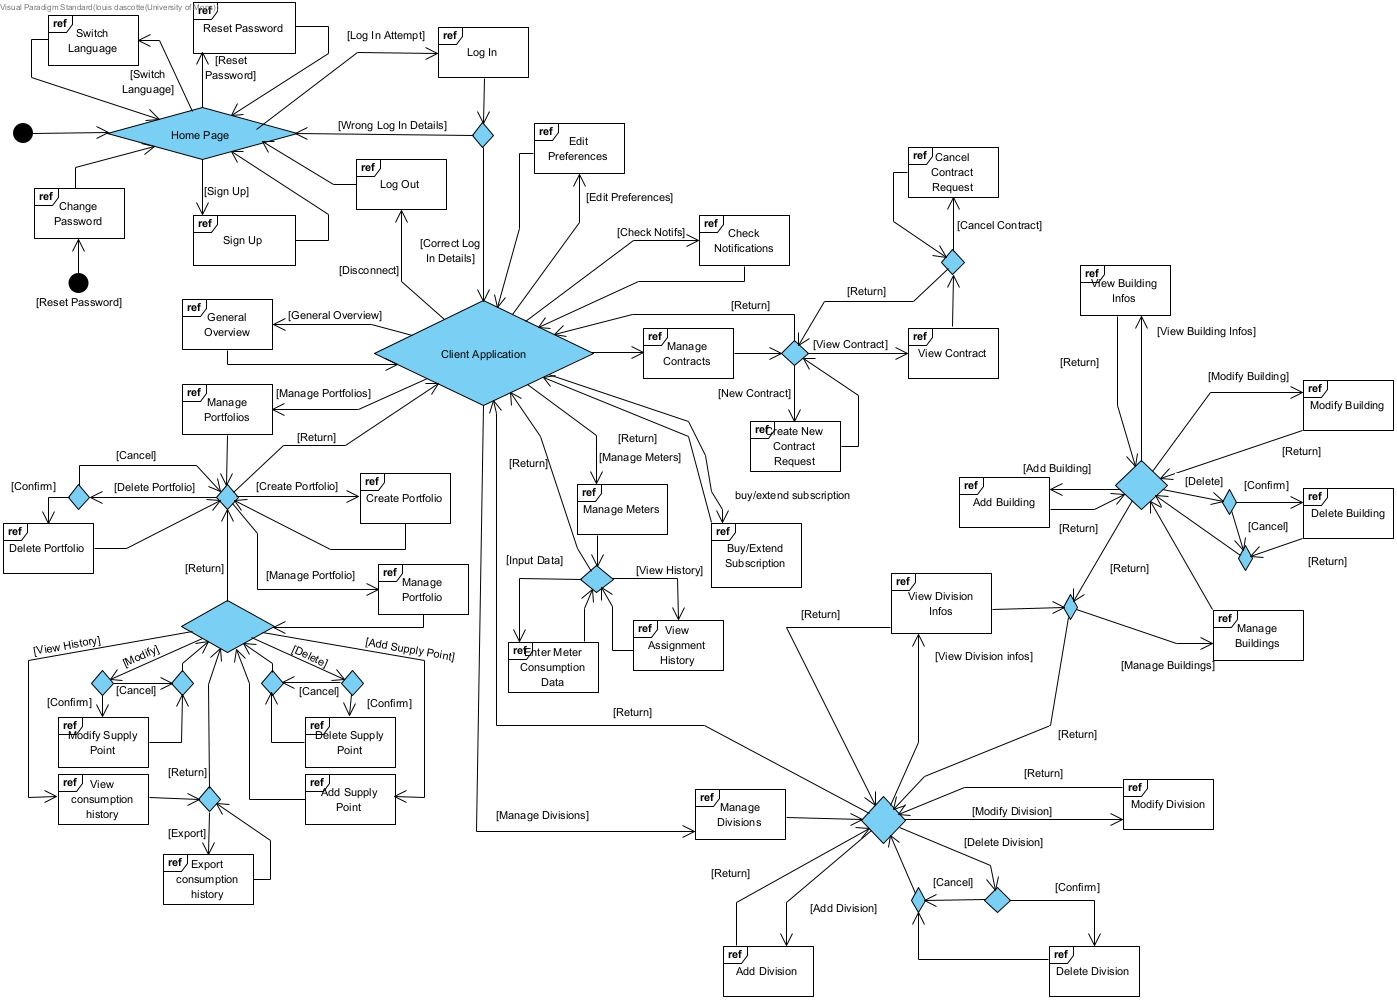
\includegraphics[width=1.3\textwidth]{IOD3}
	\caption{Interaction Overview Diagram}
	\label{fig:usdClient}
\end{figure}
\newpage
\subsection{Class Diagram}
Voici le class diagram de l'extension. Comme on peut le constater, l'organisation ressemble au compte client, mais il possède aussi des divisions.\\ Ces divisions sont représentées sous forme de comptes clients, mais ils possèdent un attribut higherUpID pour permettre de connaitre la division au dessus d'eux. Les comptes de divisions peuvent eux-mêmes avoir des sous-divisions.
\begin{figure}[h!t]
	\centering
	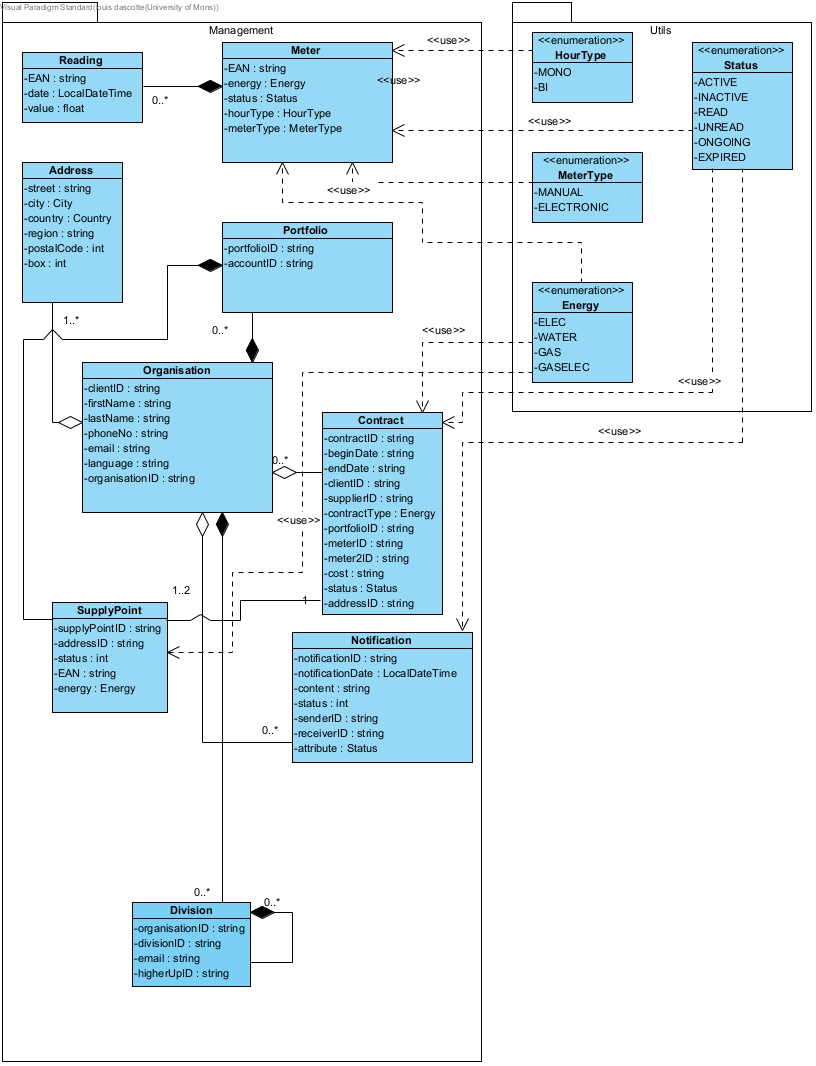
\includegraphics[width=1.3\textwidth]{GL}
	\caption{Class Diagram}
	\label{fig:ClassDiagram}
\end{figure}
\end{document}